\section{Game with a purpose (GWAP)}\label{sec:gwap}
In this section we discuss what a game with a purpose is, and why our project falls within that category. We touch on Citizen science, and how our project contributes to that. We discuss MMOS (Massively Multiplayer Online Science), and what they have done for the project. And finally we show how this project helped solve real world problems in the biological sciences. \\

\subsection{About GWAPs}
A game with a purpose, in short, is a game designed for a primary purpose other than pure entertainment. Specifically by outsourcing computational functions to humans in an entertaining way. There have been many GWAPs been released, each of them contributing in some way to real world problems such as cancer research to exoplanet discovery. 

\subsection{The purpose of our game}
Our game revolves around classifying images of immunofluorescently stained cells, these are images that researchers have taken and are stored by the \href{http://www.proteinatlas.org/}{Human Protein Atlas}. These images can not easily be classified by computers, as they lack the superior pattern recognition skills of humans. As such, non scientific humans can easily classify these images quite fast.\\ As illustrated in figure \ref{fig:outline}, the game itself receives these images from the MMOS API, displays them to the player with classification options, and distributes that image throughout the playerbase until they have reached a consensus, agreeing on the correct solution. Once a consensus has been reached, the image is considered classified and can then be used for research by scientists.\\ This is hugely beneficial to the scientific community because there are so many images (around 250 thousand) that need to be classified and it would take those few scientists years to process them all. The purpose of our game revolves around utilizing Citizen Science in an entertaining shell inside the EVE Online universe to save scientists a lot of time in classifying these images.

\begin{figure}[H]
	\centering
	\graphicspath{ {./graphics/} }
    \centerline{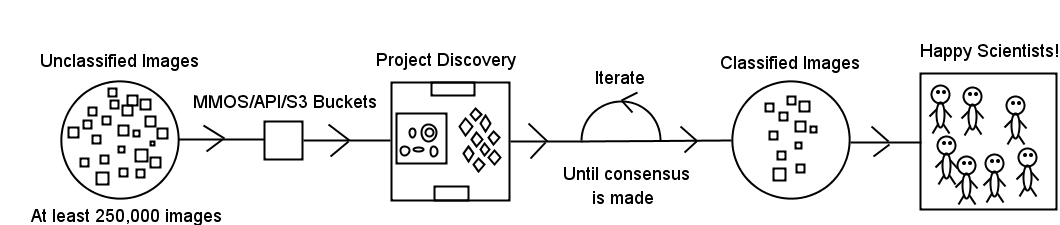
\includegraphics[width=15cm]{outline.png}}
    \caption{\label{fig:outline}The pipeline of unclassified images to scientists}
\end{figure}

\subsection{Citizen Science}
Citizen science is scientific research and analytics conducted by amateur scientists. In the online gaming scene it means classifying images, translating hand-written texts and many other useful tasks that help scientists conduct their research. In this project, players will be tasked with classifying images of immunofluorescently stained cells. This provides spatial information on protein expression patterns on a fine cellular and subcellular level. With the project implemented in to EVE Online, all of their players will have access to the project, and able to start classifying images right away. Therefore contributing to Citizen Science through his favorite online game.

\subsection{MMOS}
MMOS, or Massively Multiplayer Online Science is a start-up from Switzerland founded in 2014. The company was created by Bernard Revaz (CEO) and Attila Szantner (Head of research \& business development). MMOS is dedicated to injecting Citizen Science in to games on a massive scale. They have been a driving force behind this project and are providing as much assistance to the project as possible. What they are doing for this project is implementing an API that allows EVE Online servers to fetch and submit images from Amazon S3 buckets. This has been a huge help to the project, allowing us to focus on implementing the game client in to EVE Online.